\documentclass[tikz,border=4pt]{standalone}
\usepackage{amsmath}
\begin{document}
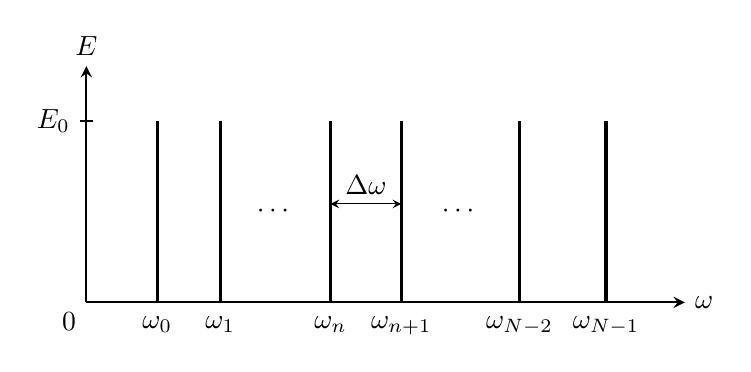
\begin{tikzpicture}[>=stealth, thick, scale=1.0]
  % Axes
  \draw[->] (0, 0) -- (7.6, 0) node[right] {$\omega$};
  \draw[->] (0, 0) -- (0, 3.0) node[above] {$E$};
  \node[below left] at (0, 0) {$0$};

  % E_0 tick
  \draw (-0.08, 2.3) -- (0.08, 2.3);
  \node[left] at (-0.08, 2.3) {$E_0$};

  % Modes with generous spacing
  \draw[very thick] (0.9, 0) -- (0.9, 2.3);
  \node[below] at (0.9, -0.05) {$\omega_0$};

  \draw[very thick] (1.7, 0) -- (1.7, 2.3);
  \node[below] at (1.7, -0.05) {$\omega_1$};

  \node at (2.4, 1.15) {$\cdots$};

  \draw[very thick] (3.1, 0) -- (3.1, 2.3);
  \node[below] at (3.1, -0.05) {$\omega_n$};

  \draw[very thick] (4.0, 0) -- (4.0, 2.3);
  \node[below] at (4.0, -0.05) {$\omega_{n+1}$};

  \draw[<->, thin] (3.1, 1.25) -- (4.0, 1.25) node[midway, above] {$\Delta\omega$};

  \node at (4.75, 1.15) {$\cdots$};

  \draw[very thick] (5.5, 0) -- (5.5, 2.3);
  \node[below] at (5.5, -0.05) {$\omega_{N-2}$};

  \draw[very thick] (6.6, 0) -- (6.6, 2.3);
  \node[below] at (6.6, -0.05) {$\omega_{N-1}$};
\end{tikzpicture}
\end{document}
